\newpage
\chapter{Implementacija}

U ovom poglavlju objašnjena je implementacija socket servera, odgovarajućeg
klijenta i na kraju samog postrojenja.
Detaljno je opisana arhitektura servera, klijenta te izrada makete postrojenja.

\section{Server}

Server je centralni dio rada. Na slici \ref{fig:main_sheme} u poglavlju
\ref{chpt:first} se vidi njegova uloga. Komunicira s postrojenjem s jedne strane
i s klijentima s druge strane. Dizajn servera se oslanja na istodobnost i
modularnost.

Glavni poslovi servera su jasno razdvojeni u različite niti. Server
sadržava tri glavne niti od koje se jedna brine oko regulacije postrojenja,
jedna prihvaćanju konekcija klijenta i jedna služi kao posrednička nit između
klijenata i regulacijske niti. Nit koja se brine oko prihvaćanju konekcija od
strane klijenta za svakog klijenta stvara novu nit te se prihvaćanje novih
konekcija može nastaviti nesmetano.

\begin{figure}[H]
\centering
\begin{tikzpicture}[every node/.style = {font=\Large\bf},
                    connection/.style = {Latex-Latex, Peach, line width=2}]
    \node[draw=OliveGreen,rectangle, rounded corners,
          fill=OliveGreen, minimum size=150]
          (regulator) {\textcolor{white}{Control thread}};

    \node[draw=MidnightBlue, rectangle, rounded corners, minimum size=150,
          right=2cm of regulator, fill=MidnightBlue]
          (server) {\textcolor{white}{Broker thread}};

    \node[draw=DarkOrchid, rectangle, rounded corners,
          minimum size=60, below left=2cm and -2.3cm of server, font=\bf\large,
          fill=DarkOrchid]
          (clientA) {\textcolor{white}{Client thread A}};

    \node[draw=DarkOrchid, rectangle, rounded corners,
          minimum size=60, right=of clientA, font=\bf\large,
          fill=DarkOrchid]
          (clientB) {\textcolor{white}{Client thread B}};

    \draw[connection] (regulator) to (server);
    \draw[connection] (server)    to (clientA);
    \draw[connection] (server)    to (clientB);
\end{tikzpicture}
\caption{Arhitektura servera}
\label{fig:architecture}
\end{figure}

Na slici \ref{fig:architecture} je prikazana komunikacija između pojedinih niti
unutar servera. Regulacijska nit, označena zelenom bojom, čita referentnu
vrijednost iz dijeljene varijable, koju postavlja posrednička nit, označena plavom
bojom, a postavlja mjerenu procesnu veličinu u drugu dijeljenu varijablu koje
klijentske niti mogu direktno očitati. Zbog zahtjeva za atomarnosti, operaciju
čitanja i pisanja dijeljenih varijabli nije moguće odobriti više od jednoj niti
zapisivanje u pojedinu dijeljenu varijablu. Zbog toga postoji posrednička nit
koja od raznih klijentskih niti preuzima referentnu vrijednost i atomarno
prosljeđuje regulacijskoj niti.

\begin{listing}[H]
\centering
\begin{minted}[frame=single]{haskell}
startDaemon :: Integer -> FilePath -> Bool -> IO ()
startDaemon port arduinoPort simulate = do
    sock <- socket AF_INET Stream 0

    bindSocket sock $ SockAddrInet (fromInteger port) iNADDR_ANY
    listen sock 50

    pv <- newMVar 0
    referenceChan <- newChan
    let com = ProcCom pv referenceChan

    _ <- forkIO $ serverLoop sock com

    controllerBroker arduinoPort simulate com
\end{minted}
\caption{Početna funkcija servera}
\label{lst:main}
\end{listing}

Na ispisu koda \ref{lst:main} prikazana je glavna funkcija, zvana
\mintinline{haskell}{startDaemon}, koja pokreće server.
Funkcija prolazi skoro kroz sve korake koji su prikazani na slici
\ref{fig:server_creation} u poglavlju \ref{subsect:haskell_net}. Prvo stvara
socket, te ga povezuje s lokalnom adresom i portom. Nakon toga se socket
pretvara u pasivni socket koji prihvaća maksimalno 50 konekcija. Nakon stvaranja
socketa i njegove pripreme, stvara se jedna dijeljena varijabla te jedan
komunikacijski kanal.

Dijeljena varijabla sadržavati će mjerenu procesnu veličinu, to jest razinu vode
u spremniku, dok će se komunikacijski kanal puniti sa željenim referentnim
veličinama od strane klijenata. Kako pojedina referentna veličina stigne od
strane klijenta, ona se stavlja u komunikacijski kanal te će ih kasnije
posrednička nit vaditi iz komunikacijskog kanala i proslijediti
regulacijskoj niti.

Na kraju se logika za socket server odvaja u novu nit sa
\mintinline{haskell}{forkIO} funkcijom koja kao argument prima
\mintinline{haskell}{serverLoop} funkciju i njene argumente. Glavna nit poziva
\mintinline{haskell}{controllerBroker} funkciju koja će nastavit s pripremom
regulacijske niti.

\begin{listing}[H]
\centering
\begin{minted}[frame=single]{haskell}
serverLoop :: Socket -> ProcCom PVType -> IO ()
serverLoop sock com = do
    (s, host) <- accept sock
    let hostinfo = show host
    noticeM rootLoggerName $ "Connected:    " ++ hostinfo
    hdl <- socketToHandle s ReadWriteMode
    _ <- forkIO $ runConn hdl com hostinfo

    serverLoop sock com
\end{minted}
\caption{Glavna serveska petlja}
\label{lst:serverLoop}
\end{listing}

Na ispisu koda \ref{lst:serverLoop} vidi se \mintinline{haskell}{serverLoop}
funkcija. Ona skupa s funkcijom \mintinline{haskell}{accept} čeka na konekciju
klijenta, a funkcija blokira sve dok se klijent ne spoji.

Za svakog klijenta koji se spoji na server ispisuje se informacija o klijentu,
socket se pretvara u handle pomoću \mintinline{haskell}{socketToHandle} funkcije,
te se stvara nova nit koja će izvršavati \mintinline{haskell}{runConn} funkciju.
Ona je zadužena za komunikaciju s klijentom te će obraditi sve zahtjeve koje
klijent pošalje. Nakon pokretanja nove niti, funkcija rekurzivno poziva samu
sebe. Rekurzivni poziv služi kao beskonačna petlja.

Socket je pretvoren u handle u \mintinline{haskell}{ReadWrite} modu i zato s
klijentima možemo komunicirati nizom standardnih IO funkcija:

\begin{itemize}
    \item \mintinline{haskell}{hGetChar :: Handle -> IO Char}
    \item \mintinline{haskell}{hGetLine :: Handle -> IO String}
    \item \mintinline{haskell}{hPutChar :: Handle -> Char -> IO ()}
    \item \mintinline{haskell}{hPutStr  :: Handle -> String -> IO ()}
\end{itemize}

Gore navedene funkcije ekvivalentne su standardnim C funkcijama:
\mintinline{haskell}{getchar}, \mintinline{haskell}{gets},
\mintinline{haskell}{putchar} i \mintinline{haskell}{puts}.

\begin{listing}[H]
\centering
\begin{minted}[frame=single]{haskell}
runConn :: Handle -> ProcCom PVType -> String -> IO ()
runConn hdl com hostinfo = do
    isEof <- hIsEOF hdl

    if isEof then do
        hClose hdl
        noticeM rootLoggerName $ "Disconnected: " ++ hostinfo
    else do
        contents <- hGetLine hdl
        debugM rootLoggerName $ "RPC request : " ++ contents

        response <- handleMsg com $ C.pack contents
        debugM rootLoggerName $ "RPC response: " ++ C.unpack response

        C.hPutStrLn hdl response
        runConn hdl com hostinfo
\end{minted}
\caption{Funkcija za klijentsku komunikaciju}
\label{lst:client_handler}
\end{listing}

Na ispisu koda \ref{lst:client_handler} nalazi se \mintinline{haskell}{runConn}
funkcija koja se brine o komunikaciji s klijentom. Komunikacija s klijentom
vrši se pomoću \mintinline{haskell}{hGetLine} i
\mintinline{haskell}{hPutStr} funkcija. Ukoliko funkcija pronađe \emph{end of
file} znak, ona zatvara handle, ispisuje informaciju o odpajanju i gasi nit. Ako
pročita čitavu liniju, string sprema u \mintinline{haskell}{contents} varijablu.

Nakon što je string spremljen, ukoliko je to poželjno, ispisuje se njegov sadržaj
te se poziva \mintinline{haskell}{handleMsg} funkcija, koja obrađuje poruku i,
ukoliko je ona valjana, izvršava određenu radnju koja je zatražena u poruci te
odgovor sprema u \mintinline{haskell}{response} varijablu. Odgovor se također
ispisuje te se šalje spojenom klijentu. Na kraju funkcija rekurzivno
poziva samu sebe kako bi bila spremna obraditi sljedeći RPC poziv.

\begin{listing}[H]
\centering
\begin{minted}[frame=single]{haskell}
controllerBroker :: FilePath -> Bool -> ProcCom PVType -> IO ()
controllerBroker arduinoPort simulate (ProcCom pvMVar refChan) = do
    refMVar <- newMVar 0

    _ <- forkIO $ forever $ do
            ref <- readChan refChan
            swapMVar refMVar ref

    if simulate then
        simulatorLoop refMVar pvMVar
    else do
        controlLoop arduinoPort refMVar pvMVar
        shutDownArduino arduinoPort

    noticeM rootLoggerName "Shutting daemon down."
\end{minted}
\caption{Posredniča funkcija}
\label{lst:controler broker}
\end{listing}

Ispis koda \ref{lst:controler broker} sadržava
\mintinline{haskell}{controllerBroker} funkciju. Ona je zadužena za pokretanje
regulacijske logike te za komunikaciju između klijenata i regulatora.

Prvo se stvara nova dijeljena varijabla. Ona će sadržavati referentnu veličinu
procesne varijable te će iz nje će regulator čitati referentnu veličinu. Stvara
se nova nit, koja čita redom referentne vrijednosti koje su postavili klijenti u
komunikacijski kanal te je postavlja u dijeljenu varijablu. Funkcija te niti
je zapakirana u \mintinline{haskell}{forever} funkciju, koja nam služi kao
beskonačna petlja.

Nakon što je posrednička i komunikacijska nit stvorena, funkcija je spremna
pokrenuti regulator. Moguće je pokrenuti simulaciju postrojenja, ukoliko Arduino
i postrojenje nisu spojeni s \mintinline{haskell}{simulatorLoop}.

Ako se ne pokrene simulacija postrojenja, pokreće se
\mintinline{haskell}{controlLoop} funkcija. U nju je implementiran jednostavni
PI regulator \cite[494]{control}. Nakon što \mintinline{haskell}{controlLoop}
funkcija završi, zbog gašenja servera ili greške pri komunikaciji s regulatorom,
poziva se \mintinline{haskell}{shutDownArduino} funkcija koja šalje
mikroupravljaču reset signal, kako bi on bio u poznatom i ugašenom stanju.

Jedine dvije funkcije koje ovise o mikroupravljaču koji se koristi su
\mintinline{haskell}{controlLoop} i \mintinline{haskell}{shutDownArduino} te se
socket server može prilagoditi bilo kojem mikroupravljaču ili procesu.

\begin{listing}[H]
\centering
\begin{minted}[frame=single]{haskell}
# ardaemon --help
Arduino control daemon 0.1

options [OPTIONS]

Common flags:
  -p --port=INT          Listnening port
  -a --arduinoport=ITEM  Path to the arduino serial port
  -s --simulate          Simulate controller
  -d --debugregulator    Enable debugging info for the regulator
  -v --verbose           Output more
  -? --help              Display help message
  -V --version           Print version information
     --numeric-version   Print just the version number
\end{minted}
\caption{Pomoćni ispis servera}
\label{lst:daemon_help}
\end{listing}

Ispis koda \ref{lst:daemon_help} prikazuje moguće opcije za pokretanje servera.
\emph{port} opcija podešava TCP port na kojem će server slušati,
\emph{arduinoport} opcija prima serijski port na kojem se nalazi arduino
mikroupravljač. Najzanimljivija opcija je \emph{simulate} opcija. Ona naređuje
serveru da pokrene simulaciju postrojenja te više ne zahtjeva arduino za rad.

Mogućnost simulacije postrojenja olakšala je izradu servera, usmjerila server ka
modularnom dizajnu i ubrzala i olakšala izradu klijenta. Simulacijska funkcija
izvšava sve bitne operacije normalne regulacijske funkcije (čitanje referentne
vrijednosti i osvježavanje trenutne vrijednosti sustava) no to čini bez senzora
i aktuatora, već je postrojenje matematički simulirano.

Slijedeće dvije opcije \emph{debugregulator} i \emph{verbose} uključuju ispis za
debugiranje regulatora ili servera. Pomoću \emph{debugregulator} regulacijska nit
ispisuje informacije o stanju sustava i regulatora za svaku iteraciju
regulacijske petlje, dok \emph{verbose} opcija ispisuje informacije o primljenim
RPC-pozivima te odgovarajućim odgovorima.

Ostale tri opcije \emph{help}, \emph{version} i \emph{numeric-version} ispisuju
samo informacije o serveru te ne pokreću server. \emph{help} ispisuje
informacije o serveru viđene na ispisu koda \ref{lst:daemon_help},
\emph{version} ispisuje ime i trenutnu verziju servera dok
\emph{numeric-version} ispisuje samo trenutnu verziju.

\newpage
\section{Klijent}

Klijent je najatraktivniji dio rada za korisnike. On korisniku preko grafičkog prikaza
omogućuje uvid u stanje postrojenja u stvarnom vremenu i lagano
upravljanje postrojenjem. Klijent je pisan u Pythonu i pomoću asinkronog
programskog modela omogućen je grafički prikaz, koji je reaktivan te ne blokira
izvođenje programa u niti jednom trenutku.

\begin{listing}[H]
\centering
\begin{minted}[frame=single]{py3}
def main():
    sock = socket.socket(socket.AF_INET, socket.SOCK_STREAM)
    sock.connect((args.host, args.port))

    tank = TankWidget()
    command_line = CommandLine(cmd_list, remote_cmds, sock)
    top = urwid.Frame(tank, None, command_line, 'footer')

    evl = urwid.AsyncioEventLoop(loop=asyncio.get_event_loop())
    loop = urwid.MainLoop(top, palette, event_loop=evl)

    loop.watch_file(sock.fileno(), read_cb)
    loop.set_alarm_in(0.1, periodic_tasks)

    loop.run()
\end{minted}
\caption{Početna funkcija klijenta}
\label{lst:client main}
\end{listing}

Ispis koda \ref{lst:client main} sadržava main funkciju klijenta. Funkcija
započinje stvaranjem socketa te se odmah spaja na server. Nakon spajanja
slijedi inicijalizacija grafičkih elemenata. Grafičko sučelje sastoji se od dva
grafička elementa: \mintinline{py3}{TankWidget} i \mintinline{py3}{CommandLine}.

\mintinline{py3}{TankWidget} zadužen je za iscrtavanje shematskog prikaza
postrojenja. Iscrtava shemu spremnika vode i njegovo trenutno stanje. Za
iscrtavanje koristi Unicode-Brailleove znakove, koji su se pojavili u 3.0 verziji
Unicode standarda \cite{unicode}.

\mintinline{py3}{Commandline} stvara komandnu liniju koja je zadužena za
primanje naredbi od strane korisnika te ih izvršava sam ukoliko su lokalne
naredbe ili ih prosljeđuje serveru preko socketa. Komandna linija podržava
standardne \emph{Emacs} kratice i upotpunjavanje naredbi pomoću \emph{tab}
tipke.

Nakon inicijalizacije grafičkog sučelja stvara se event loop te se dodaje ranije
stvoreni socket na listu praćenih događaja pomoću \mintinline{py3}{read_cb()}
funkcije, koja se poziva ukoliko podatci stignu na socket. Također se dodaje
vremenski događaj koji će pozvati \mintinline{py3}{periodic_tasks()} funkciju
nakon 0.1 sekunde nakon što se event loop počne izvršavati. Ona je zadužena za
periodičko osvježavanje stanja postrojenja.

Na kraju se samo još pokreće event loop koji će se izvršavati sve dok korisnik,
pomoću komandne linije, ne preda naredbu za gašenje programa.

\begin{listing}[H]
\centering
\begin{minted}[frame=single]{py3}
    def periodic_tasks(loop, data):
        request , _ = lvl_cmd('update-tank', [])
        try:
            sock.send(bytes(request, 'utf-8'))
        except BrokenPipeError as e:
            pass

        tank.update()

        loop.set_alarm_in(args.interval, periodic_tasks)
\end{minted}
\caption{Funkcija periodičkih poslova}
\label{lst:periodic tasks}
\end{listing}

Na ispisu koda \ref{lst:periodic tasks} vidljiva je
\mintinline{py3}{periodic_tasks()} funkcija. Ona stvara RPC poziv pomoću
\emph{update-tank} metode te ga šalje serveru preko socketa.

Nakon slanja RPC poziva poziva \mintinline{py3}{update()} metodu
\emph{TankWidget} grafičkog elementa. Ukoliko je došlo do promjene u stanju
postrojenja, ona osvježava iscrtavanje njegovog shematskog prikaza.

Na kraju se još dodaje novi vremenski događaj koji će ponovno pozvati
\mintinline{py3}{periodic_tasks()} funkciju. Interval tih periodičkih
poslova korisnik može namjestiti na
komandnoj liniji pri pokretanju klijenta.

\begin{listing}[H]
\centering
\begin{minted}[frame=single]{haskell}
# arclient --help
optional arguments:
  --help                show this help message and exit
  --port PORT           port to use (Default 4040)
  --host HOST           host to connect to (Default localhost)
  --interval INTERVAL   update interval
\end{minted}
\caption{Pomoćni ispis klijenta}
\label{lst:client_help}
\end{listing}

Na ispisu koda \ref{lst:client_help} prikazane su moguće opcije pri pokretanju
klijenta. \emph{help} opcija ispisuje informacije o klijentu viđene na ispisu
koda \ref{lst:client_help}, \emph{port} opcija postavlja korišteni TCP port pri
spajanju na server, \emph{host} opcija postavlja adresu koja će se koristiti pri
spajanju i \emph{interval} opcija postavlja interval za osvježavanje stanja
sustava i grafičkog sučelja.

\begin{figure}[H]
\centering
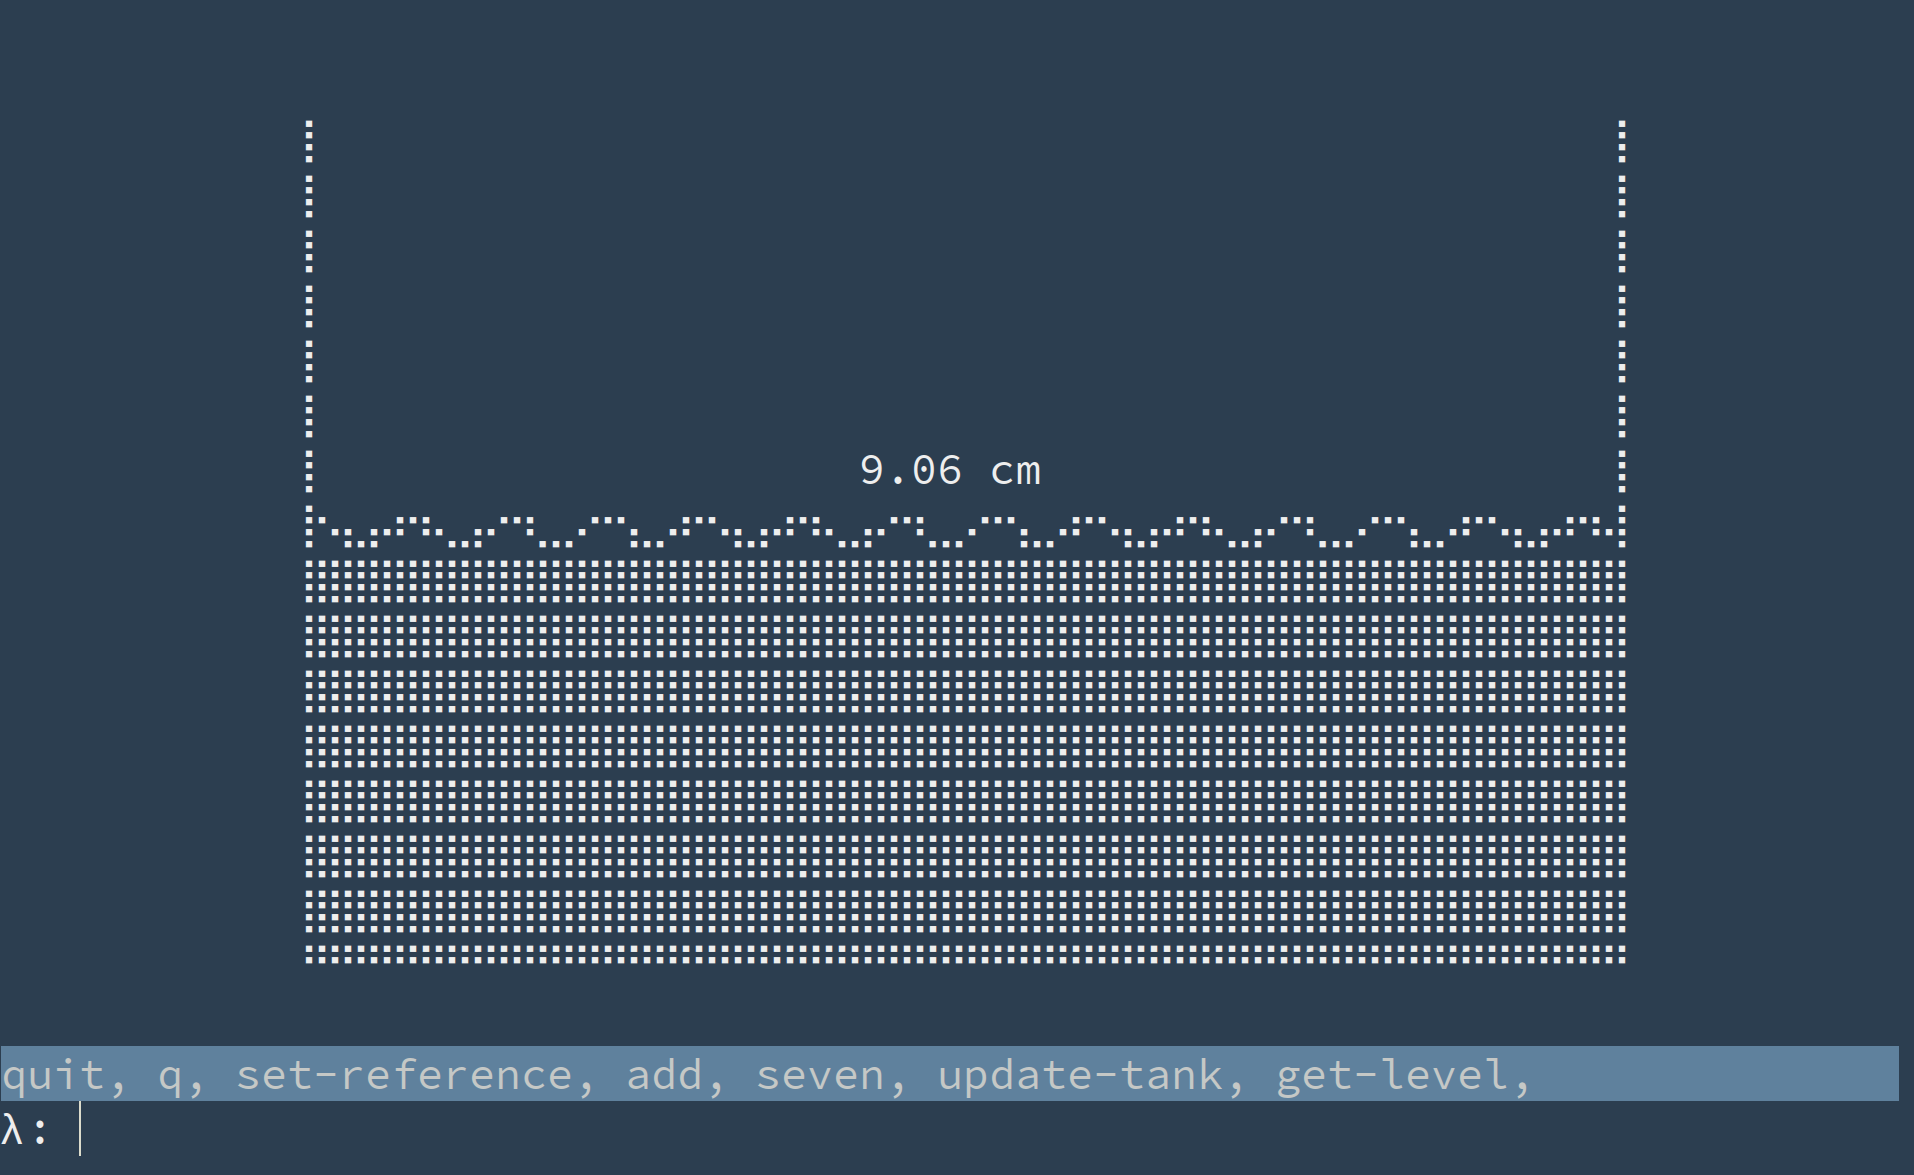
\includegraphics[scale=0.25]{figures/arclient-2.png}
\caption{Prikaz klijenta}
\label{fig:client}
\end{figure}

Na slici \ref{fig:client} je prikazano grafičko sučelje klijenta. Gornji dio
grafičkog sučelja prikazuje shematski prikaz spremnika vode i razinu vode u
stvarnom vremenu. Iznad razine vode ispisana je zadnje izmjerena razina vode.

Ispod shematskog prikaza spremnika vode nalazi se informacijski dio komandne
linije, to jest statusna linija gdje su trenutno ispisane sve podržane naredbe:
\begin{itemize}
    \item quit
    \item q
    \item set-reference
    \item add
    \item seven
    \item update-tank
    \item get-level
\end{itemize}

Naredbe su odvojene u lokalne i udaljene naredbe. Lokalne naredbe su: \emph{quit}
i \emph{q}. Naredba \emph{quit} služi za gašenje klijenta, a naredba \emph{q}
samo je alias na naredbu \emph{quit}.

Udaljene naredbe su: \emph{set-reference}, \emph{add}, \emph{seven},
\emph{update-tank}, \emph{get-level}. Sve udaljene naredbe generiraju JSON-RPC
poziv te ga šalju serveru i registriraju funkcije koje će obraditi odgovor kad
on stigne.

Naredba \emph{set-reference} je najvažnija naredba klijenta. Ona nam omogućuje
promjenu referentne vrijednosti u stvarnom vremenu. Kao argument prima razinu
vode u boci te ga spremi u JSON-RPC poziv. Ukoliko dolazi do greške, greška se
ispisuje u statusnoj liniji.

Naredba \emph{add} je testna naredba koja prima dva brojčana argumenta te ih
šalje serveru u JSON-RPC pozivu. Server će zbrojiti primljene brojčane argumente
i rezultat zbrajanja poslati natrag u JSON-RPC odgovoru. Nakon što odgovor
stigne, njegov rezultat bit će prikazan u statusnoj liniji.

Naredba \emph{seven} također je testna naredba. Ona serveru šalje, unutar
JSON-RPC poziva, broj sedam. Server u JSON-RPC odgovoru šalje istu brojčanu
vrijednost natrag. Naredba služi kao jednostavni \emph{echo} test. Rezultat
odgovora prikazuje se u statusnoj liniji.

\emph{update-tank} naredba je naredba koja se izvršava automatski kao dio
periodičkih zadataka koje event loop obavlja. Naredba dohvaća trenutnu razinu
postrojenja te ga prosljeđuje \mintinline{py3}{TankWidget} grafičkom elementu
koji osvježava iscrtavanje shematskog prikaza, ukoliko je došlo do promjene.
\emph{get-level} naredba šalje isti JSON-RPC poziv kao i \emph{update-tank}
naredba, no umjesto da trenutnu razinu proslijedi grafičkom elementu za prikaz, ona
razinu jednostavno prikaže u statusnoj liniji.

Ispod statusne linije nalazi se sama komandna linija u koju je moguće prije
navedene naredbe upisati.

\newpage
\section{Postrojenje}

Postrojenje je napravljeno u obliku makete spremnika u kojem se održava razina
vode. Ulazni tok u spremnik ostvaren je pomoću vodene pumpe čijom se brzinom
može upravljati pomoću pulsno širinske modulacije. Izlazni tok spremnika
ostvaren je pomoću otvora pri dnu spremnika te voda slobodnim padom teče iz
spremnika. Razina u spremniku direktno se mjeri pomoću senzora.

\begin{figure}[H]
\centering
\begin{tikzpicture}[every node/.style = {font = \footnotesize}]
    \tikzset{weird fill/.style={append after command={
    \pgfextra
        \draw [#1, sharp corners, fill=#1]%
        (\tikzlastnode.west)%
        [rounded corners=0] |- (\tikzlastnode.north)%
        [rounded corners=3] -| (\tikzlastnode.east)%
        [rounded corners=0] |- (\tikzlastnode.south)%
        [rounded corners=0] -| (\tikzlastnode.west);
        \endpgfextra}}}

    \draw [rounded corners=3] (-5,10) -- (-2,10) -- (-2,9);
    \draw [rounded corners=3] (-5,10.5) -- (-1.5,10.5) -- (-1.5,9);
    \draw (-1.75, 9) circle [x radius=0.25, y radius=0.05];
    \draw (-4, 10.25) node [font=\normalsize] {$q_{in}$};
    \draw [-Latex, thick] (-3.5, 10.25) -- (-2.5, 10.25);

    \draw (0, 2.5) node[rectangle, minimum width=228, minimum height=140,
    fill=NavyBlue] {};

    \draw [fill=NavyBlue] (0,0) circle [x radius=4, y radius=0.5];
    \draw [fill=NavyBlue, thick, dashed] (0,5) circle [x radius=4, y radius=0.5];

    \node [font=\large] (area) {\textcolor{white}{$A$}};
    \node [font=\large, above=4.4 of area] {\textcolor{white}{$V$}};

    \draw (4,9)  arc[x radius = 4, y radius = 0.5, start angle=0, end angle=112];
    \draw (4,9)  arc[x radius = 4, y radius = 0.5, start angle=0, end angle=-240];

    \draw (-4,0)  -- (-4,9);
    \draw (4,0)   -- (4,0.5);
    \draw (4,1.2) -- (4,9);

    \draw (4.9, 0.85)
    node[weird fill=NavyBlue, rectangle, minimum width=62, minimum height=19]
    (qout1) {};
    \draw (4.5, 0.85) node [font=\normalsize] {\textcolor{white}{$q_{out}$}};

    \node [below right=-0.1 and -0.7 of qout1, fill=NavyBlue, minimum width=20, minimum
    height=17] (qout2) {};

    \draw [NavyBlue, fill=NavyBlue] (5.2, 0.6) -- (5.2,0.7) -- (5.5,0.7) -- (5.30, 0.4);
    \draw [NavyBlue, fill=NavyBlue] (5.2, 0.6) -- (5.2,0.5) -- (5.5,0.49);
    \draw [rounded corners=3] (4,1.2) -- (6,1.2) -- (6,0);
    \draw [rounded corners=3] (4,0.5) -- (5.3,0.5) -- (5.3,0);

    \draw [fill=NavyBlue] (5.65,0) circle [x radius=0.35, y radius=0.05];

    \draw (-4, 0) -- (-4.5, 0);
    \draw (-4, 5) -- (-4.5, 5);
    \draw [Latex-Latex] (-4.5, 0) -- (-4.5, 5);
    \draw (-4.7, 2.5) node [font=\large] {$h$};

\end{tikzpicture}
\caption{Shematski model postrojenja}
\label{fig:plant}
\end{figure}

Na slici \ref{fig:plant} vidi se postrojenje. Iznad glavnog spremnika vidi se
ulazna cijev s ulaznim tokom $q_{in}$, dok se u desnom dijelu glavnog spremnika
nalazi otvor za izlazni tok $q_{out}$.

Razina vode u spremniku označena je s $h$, dok je volumen koji voda zauzima u
spremniku označen s $V$. Površina poprečnog presjeka spremnika označena je s
$A$.

\newpage
\subsection{Matematički model postrojenja}


Volumen vode u spremniku ovisi o ulaznom toku i izlaznom toku. Volumen će ostati
konstantan, ukoliko su ulazni i izlazni tok isti, dok će se volumen vode mijenjati
ovisno o razlici ulaznog toka i izlaznog toka te stoga možemo reći:

\begin{equation}
    \frac{dV}{dt} = q_{in} - q_{out}
\label{eq:first}
\end{equation}

Gdje je ulazni tok definiran kao:

\begin{equation} q_{in} = k_p U \end{equation}

gdje je:
\begin{description}[labelindent=2cm]
        \item[$k_p$] - konstanta pumpe
        \item[$U$]   - napon pumpe
\end{description}

Izlazni tok je određen pomoću Torricellijevog zakona \cite[75]{fluid}:

\begin{equation} q_{out} = a \sqrt{2gh} \end{equation}

gdje je:
\begin{description}[labelindent=2cm]
        \item[$a$] - poprečni presjek izlazne cijevi
        \item[$g$] - ubrzanje zemljine sile teže
            (\unit{9.80665}{\metre\per\square\second})
        \item[$h$] - visinska razina vode u spremniku
\end{description}

Budući da je spremnik cilindričnog oblika, za volumen spremnika možemo uzeti
jednakost $V = A h$. Uvrštavanjem ulaznog i izlaznog toka te jednakosti za
volumen u jednadžbu \ref{eq:first} dobiva se:

\begin{equation}
    A\frac{dh}{dt} = k_p U - a \sqrt{2gh}
\label{eq:nonlin}
\end{equation}

Iz jednadžbe \ref{eq:nonlin} je vidljivo da ona sadržava nelinearni element u obliku
$a \sqrt{2gh}$. Kako bi uspješno mogli analizirati sustav i primijeniti Laplaceovu
transformaciju, jednadžba koja opisuje sustav mora biti linearizirana
\cite[88-97]{control}:

\begin{equation} \frac{d\delta h}{dt} = \frac{k_p}{A} \delta U -
                 \frac{a \sqrt{2g}}{2 A \sqrt{h_0}} \delta h \end{equation}

gdje je:
\begin{description}[labelindent=2cm]
        \item[$h_0$] - radna točka oko koje je sustav lineariziran
\end{description}

Konstantne vrijednosti, uz $\delta U$ i $\delta h$, mogu se jednostavnosti radi
staviti u poseban izraz:

\begin{equation}
    \frac{d\delta h}{dt} = k_1 \delta U - k_2 \delta h
\end{equation}

Sada se može primijeniti Laplaceova transformacija \cite[35-44]{control} pri čemu
se dobiva:
\begin{equation} s H(s) = k_1 U(s) - k_2 H(s) \end{equation}

Nakon grupiranja $H(s)$ elemenata na lijevoj strani jednadžbe, dobiva se:
\begin{equation} H(s)(s+k_2) = k_1 U(s) \end{equation}

Te konačno se dobiva prijenosna funkcija sustava \cite[45]{control}:
\begin{equation}
    G(s) = \frac{H(s)}{U(s)} = \frac{k_1}{s+k_2}
\label{eq:transfer}
\end{equation}

Iz jednadžbe \ref{eq:transfer} je vidljivo da jednadžba predstavlja sustav prvog
reda \cite[166]{control}. Osim što je sustav poprilično jednostavan, on je i samo
stabilizirajući \cite{control_guru}, tj. za svaku ulaznu veličinu sustav će se
nakon određenog vremena stabilizirati.

Zbog jednostavnosti sustava možemo odabrati jednostavni PI regulator koji će
omogućiti brz dolazak u stacionarno stanje te smanjiti regulacijsku grešku
stacionarnog stanja.

\subsection{Senzor i aktuator}

Da bi regulator mogao obavljati svoj posao, mora imati uvid u stanje sustava te
mora imati način na koji promijeniti stanje. Uvid u stanje regulatoru pruža senzor
razine tekućine, a promjena stanja moguća je pomoću pumpe tekućine.

Za senzor je korišten \emph{eTape} senzor razine tekućine \cite{etape}. Senzor
je realiziran kao promjenjivi otpornik, čiji se otpor mijenja ovisno na kojem
dijelu senzora hidrostatski tlak tekućine pritišće senzora. Izlazni otpor senzora
obrnuto je proporcionalan razini tekućine.

Radi veće preciznosti mjerenja, izlazni otpor senzora pretvara se u napon raspona
od \unit{0-5}{\volt}. Pretvorba izlaznog otpora u napon ostvarena je pomoću
\emph{\unit{0-5}{\volt} Linear Resistance to Voltage Module} istog proizvođača
kao i senzora \cite{voltage_module}.

\begin{table}[h]
\caption{Kalibracijske vrijednosti senzora}
\setlength{\tabcolsep}{14pt}
\centering
    \begin{tabular}{|c|c|c|c|c|c|c|c|}
        \hline
        Napon (\volt) &
        0.36  &  0.56  &  0.78  & 1.01  & 1.19  & 1.40 &  1.66 \\
        \hline
        Razina vode (\centi\metre) &
        4  &  5  &  6  &  7  &  8  &  9  & 10 \\
        \hline
        \hline
        Napon (\volt) &
        1.85  &  2.05  &  2.25  & 2.53  & 2.83  & 2.97 &  3.26 \\
        \hline
        Razina vode (\centi\metre) &
        11  & 12  & 13 &  14 &  15&16 &  17 \\
        \hline
    \end{tabular}
    \label{tbl:etape}
\end{table}

U tablici \ref{tbl:etape} se nalaze mjerene naponske vrijednosti senzora uz
određene razine vode. Senzor ima mrtvi pojas od \unit{0-2.54}{\centi\metre}, u
kojem se otpor te u konačnici napon ne mijenjaju.

\begin{figure}[H]
\centering
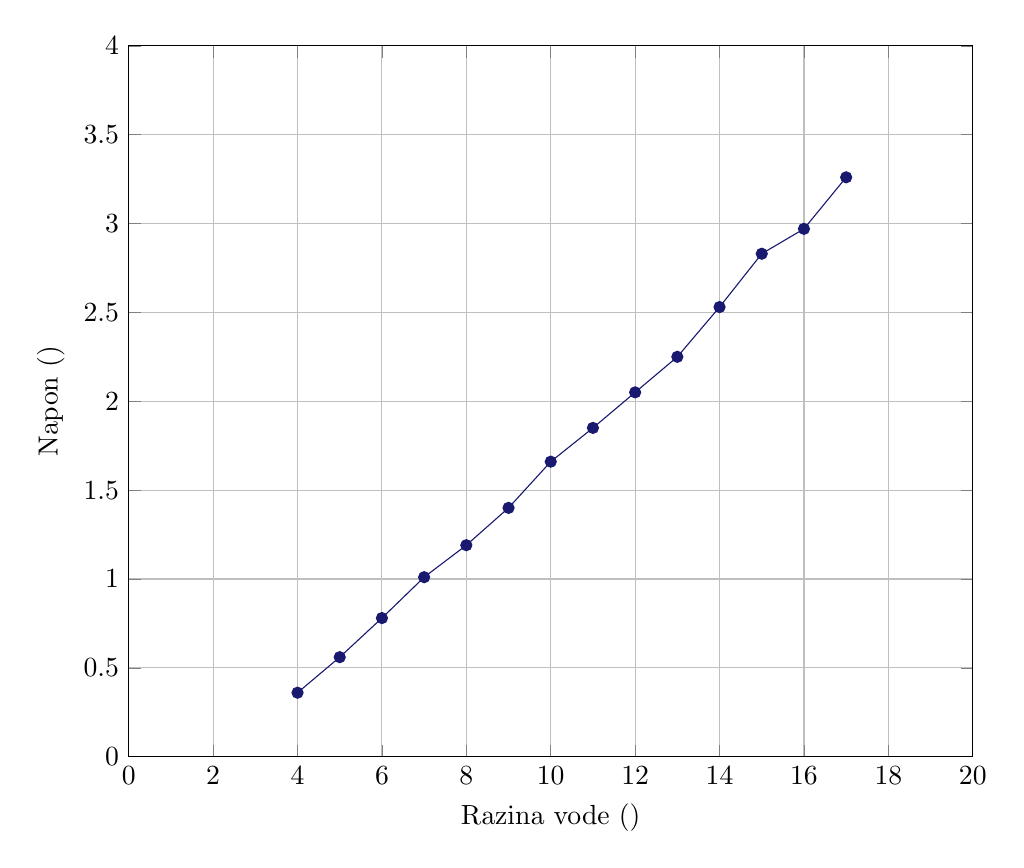
\begin{tikzpicture}
    \begin{axis}[width=350, xlabel=Razina vode (\centi\metre), ylabel=Napon
                 (\volt), grid=major, ymin=0, ymax=4, xmin=0, xmax=20]
    \addplot[color=MidnightBlue, mark=*] coordinates {
        (4, 0.36)
        (5, 0.56)
        (6, 0.78)
        (7, 1.01)
        (8, 1.19)
        (9, 1.4)
        (10, 1.66)
        (11, 1.85)
        (12, 2.05)
        (13, 2.25)
        (14, 2.53)
        (15, 2.83)
        (16, 2.97)
        (17, 3.26)
    };
    \end{axis}
\end{tikzpicture}
\caption{Graf odziva senzora}
\label{fig:etape}
\end{figure}

Na grafu \ref{fig:etape} se vidi promjena napona ovisno o razini vode. Jasno je
vidljiv linearni odziv senzora.

Pumpa koja je odabrana je mala pumpa za modelske svrhe maksimalnog protoka od
\unit{1.84}{\litre\per\minute}. Protok pumpe se može regulirati naponski.
Minimalni napon pumpe je \unit{3}{\volt}, a maksimalni \unit{12}{\volt}.

\begin{table}[h]
\caption{Kalibracijske vrijednosti pumpe}
\setlength{\tabcolsep}{14pt}
\centering
    \begin{tabular}{|c|c|c|c|c|c|c|}
        \hline
        Napon (\volt) & 12 & 10 & 8 & 5 & 4 & 3 \\
        \hline
        Protok (\centi\cubic\metre\per\second) &
        28.8889 & 23.3332 & 18.4193 & 11.3328 & 8.1663 & 5.0008 \\
        \hline
    \end{tabular}
    \label{tbl:pump}
\end{table}

U tablici \ref{tbl:etape} se nalazi mjereni protok pumpe senzora uz
određene naponske razine.

\begin{figure}[H]
\centering
\begin{tikzpicture}
    \begin{axis}[width=350, xlabel=Napon (\volt), ylabel=Protok
                 (\centi\cubic\metre\per\second), grid=major, xmin=0, xmax=14,
                 ymin=0, ymax=30]
    \addplot[scale=2, color=MidnightBlue, mark=*] coordinates {
        (3, 5.0008)
        (4, 8.1663)
        (5, 11.3328)
        (8, 18.4193)
        (10, 23.3332)
        (12, 28.8889)
    };
    \end{axis}
\end{tikzpicture}
\caption{Graf odziva pumpe}
\label{fig:pump}
\end{figure}

Na grafu \ref{fig:pump} se vidi promjena protoka pumpe ovisno o naponskoj
razini. Zbog ograničenog maksimalnog protoka pumpe, brzina odziva sustava ovisi o
veličini spremnika. Za relativno brz odziv sustava odabrana je boca volumena od
\unit{1}{\litre}. Boca je cilindričnog oblika, radijus joj je
\unit{4}{\centi\metre}, a visina nešto ispod \unit{20}{\centi\metre}. Zbog
mrtvog pojasa senzora regulacija ispod \unit{3}{\centi\metre} nije moguća.

\newpage
\subsection{Arduino shield}

Operativni napon izlazno/ulaznih pinova Arduino mikroupravljačke pločice je u
rasponu od \unit{0-5}{\volt} te nije u stanju iskoristiti čitav operativni
raspon pumpe. Da bi se mogao iskoristiti čitav operativni raspon pumpe koristi
se \emph{L293E} integrirani krug za pogon istosmjernih motora \cite{h-bridge}.

\begin{figure}[H]
\centering
\includegraphics[scale=0.80]{figures/shield_schematic.pdf}
\caption{Električna shema postrojenja}
\label{fig:schematic}
\end{figure}

Slika \ref{fig:schematic} prikazuje potpunu električnu shemu postrojenja gdje
je:
\begin{description}[labelindent=2cm]
        \item[IC1] - Arduino mikroupravljačka pločica
        \item[IC2] - L293E IC za pogon istosmjernih motora
        \item[IC3] - Modul koji pretvara otpor senzora u napon
        \item[S]   - \emph{eTape} senzor razine tekućine
        \item[P]   - \unit{12}{\volt} pumpa
        \item[D1]  - zaštitna dioda
        \item[C1]  - stabilizacijski kondenzator
\end{description}

Shema također prikazuje spojeve između svih komponenti postrojenja. Analogni
ulaz Arduina A0 spojen je na izlaz IC3 modula. Arduino na analognom ulazu A0
prima \unit{0-5}{\volt} signal koji je proporcionalan razini vode. Na
\emph{L293E} integriranom krugu su pinovi za pogon prvog i četvrtog kanala
kratko spojeni te se opterećenje tijekom rada raspodjeljuje na oba kanala.

Digitalni pin D2, koji je konfiguriran kao izlaz, spojen je na \emph{Chip Enable}
pin \emph{L293E} integriranog kruga. Njime se upravlja aktivacija pogonskih
kanala integriranog kruga. Napon na izlazu \emph{L293E} integriranog kruga ovisi
o naponu na ulazu. Ulaznim naponom upravljamo pomoću izlaznog pina D3 na
Arduinu.

D3 pin Arduina konfiguriran je kao pulsno širinski izlazni pin. Izlazni
pin \emph{L293E} integriranog kruga spojen je na pumpu. Paralelno s pumpom u
spoju je dioda D1. Ona štiti strujni krug od induktivnog napona koji se pojavljuje
pri gašenju pumpe.

\subsection{Regulator}

Regulator, koji je dio servera, komunicira s Arduinom te pomoću Arduina upravlja
postrojenjem. Osnovna mu je zadaća primiti željenu referentnu vrijednost te
sustav dovesti u novo, stacionarno stanje i zadržati ga ondje.

Radi jednostavnosti i niskog reda sustava, kao regulator odabran je PI
regulacijski algoritam.

\begin{listing}[H]
\centering
\begin{minted}[frame=single]{haskell}
forever $ do
    reference <- liftIO $ readMVar refMVar
    integral  <- liftIO $ takeMVar integralMVar

    sensorValue <- analogRead sensor
    let fillHeight = sensorValueFunc sensorValue
    _ <- liftIO $ swapMVar pvMVar fillHeight
    let error = reference - fillHeight

    let proportional_term = kp * error
    let integral_term     = integral + ki * error / sampleTime
    liftIO $ putMVar integralMVar integral_term

    let output = clampAndScaleOutput $ proportional_term + integral_term

    analogWrite pwm_pin output
    delay sampleTime
\end{minted}
\caption{Regulacijska petlja}
\label{lst:regulator}
\end{listing}

Na ispisu koda \ref{lst:regulator} prikazana je regulacijska funkcija koja se
nalazi unutar servera. Prvo se uzima referenca i vrijednost integratora iz dijeljenih varijabli.
\mintinline{haskell}{integralMVar} je interna varijabla regulatora gdje se
sprema akumulirana vrijednost integratora, dok je \mintinline{haskell}{refMVar}
dijeljena varijabla u koju posrednička funkcija stavlja referentnu vrijednost.

Odmah nakon čitanja dijeljenih varijabli, od Arduina se traži trenutna
razina vode pomoću \mintinline{haskell}{analogRead} funkcije. Razina se pretvara
iz naponske vrijednosti u visinu pomoću \mintinline{haskell}{sensorValueFunc} te
se sprema u \mintinline{haskell}{fillHeight} varijablu i prosljeđuje ostatku
servera, spremajući je u za to namijenjenu dijeljenu varijablu.

Nakon što je mjerenje izvršeno i trenutna referentna vrijednost preuzeta,
pomoću istih se računa odstupanje od referentne vrijednosti te se sprema u
\mintinline{haskell}{error} varijablu. Integralni dio regulatora sprema se u
prije spomenutu varijablu \mintinline{haskell}{integralMVar}, koja će ju
sačuvati za sljedeću iteraciju regulacijske petlje.

Sada se mogu proporcionalni i integralni članovi regulatora izračunati i
zbrojiti. Funkcija \mintinline{haskell}{clampAndScaleOutput} ograničava izlaz
regulatora na operativni raspon pumpe i brine se o tome da pumpa ne pokušava
raditi na naponu ispod \unit{3}{\volt}.

Preostaje samo poslati novu naponsku razinu na Arduino, a on će ju primijeniti na
pulsno širinskom pinu i tako postaviti protok pumpe. Nakon toga petlja čeka
određeno vrijeme te ponovno izvršava sve navedene korake.

\begin{figure}[H]
\centering
\begin{tikzpicture}
    \begin{axis}[width=350, xlabel=Vrijeme (\second), ylabel=Razina vode
                 (\centi\metre), grid=major, xmin=0, xmax=120,
                 ymin=0, ymax=20]
                 \addplot[samples=100, domain=0:120, dashed] { 15 };
                 \addplot[MidnightBlue, very thick]
                    table [x=time, y=height, col sep=comma] {regulator_response.csv};
    \end{axis}
\end{tikzpicture}
\caption{Graf odziva regulatora}
\label{fig:step_response}
\end{figure}

Na slici \ref{fig:step_response} je prikazan izmjereni odziv regulatora uz $k_p = 4$ i
$k_i = 1.5$.
